\documentclass[twocolumn]{revtex4}
\usepackage{graphics,graphicx,epsfig,ulem,amsmath,multirow,gensymb,commath,textcomp,natbib}
\newcommand{\squeezeup}{\vspace{-2.5mm}}

\begin{document}

\textheight=26.385cm
%Change textheight as the last resort...

\title{Investigating and understanding Fraunhofer diffraction patterns using Fourier analysis with variations of the 4f Optical System}
 
\author{Jacky Cao, Room 205, Friday, Lab Partners: Thomas Spriggs \\ Date of experiment: 10/02/2017 to 17/03/2017, Date of report: 19/03/2017}

\begin{abstract}              
Through the study of the Fourier Transforms of blah blah blah. \cite{crc}. 
\end{abstract}

\maketitle

\section{Introduction} 
\vspace{-2ex} 

In the field of optics, a Fraunhofer diffraction pattern can be produced when a coherent beam of radiation falls onto a partially opaque object \cite{mathmethods}. The pattern can then be viewed at a ``far-field'' distance, this length being larger than the initial size of the object, allowing for the spreading of light due to diffraction to dominate in the observation plane \cite{of2f}. 

The usage of diffraction patterns includes the studying of crystalline structures. Through X-ray and electron diffraction it is possible to obtain accurate information about the identity of phases present, atomic ordering, and for recognising different metallurgical constituents within a specimen. This allows for potential applications within the pharmaceutical industry for example, where early analysis of different mixtures and compounds can be cost and time saving. \cite{elecdiffraction, xraypharma}

Another application could potentially involve using the diffraction pattern within an illumination system so that x-ray phase contrast microscopy and interferometry can be performed \cite{singleslit}. This could be used to enhance the visibility of fine scale structures, this being especially useful in biology as quantitative information can be obtained about a sample from just phase-contrast images \cite{xrayphase}.

With these varying applications we find that in order to fully understand diffraction patterns and how they form, we must look at the mathematics behind them. 

The main mathematical tool that we must use in building our understanding is Fourier analysis, more specifically, Fourier transforms. A Fourier transform is a way to represent a function in terms of a superposition of sinusoidal functions, with the explicit conditions of the function being defined over an infinite interval and having no particular periodicity \cite{mathmethods}.

The Fourier transform $F(u)$ of a single function $f(x)$ can be stated as,
\begin{equation}
F(u) = \mathcal{F}[f(x)](u) = \int_{-\infty}^\infty f(x) e^{-i2\pi ux}dx,
\label{fourierdefinition}
\end{equation}

where $(u)$ is the dependent Fourier variable. This expression tells us the spectrum of frequencies required to form the function $f(x)$ \cite{of2f}.

We can also operate on the initial function then Fourier transform it. In Table \ref{fourierproperties} we find the group of functions known as the Fourier transform properties.
\begin{table}[h!]
\centering
\begin{tabular}{c@{\hskip 20pt}c@{\hskip 20pt}c@{\hskip 20pt}c} 
 \hline
 \textbf{Property} & \textbf{$\boldsymbol{f}$} & \textbf{$\boldsymbol{F}$} \\ [0.5ex] 
 Linearity				& $g(x)+h(x)$ & $G(u) + H(u)$ \\
 Translation 			& $f(x-a)$ 	& $F(u)e^{-i2\pi ua}$ \\ 
 Scaling 				& $f({x/a})$ & $aF(ua)$ \\
 Convolution			& $(g*h)(x)$ & $GH$ \\
 Inverse Convolution		& $gh$ & $ (G*H)(u)$ \\
 \hline
\end{tabular}
\caption{The Fourier transform properties - different functions $\boldsymbol{f}$ and their output $\textbf{$\boldsymbol{F}$}$ when they have been Fourier transformed using equation \ref{fourierdefinition}.}
\label{fourierproperties}
\end{table}

The convolution property can be better understood as follows - if we convolve two functions of $x$, $g(x)$ and $h(x)$, then that is defined as,
\begin{equation}
(g*h)(x) = \int_{-\infty}^\infty g(x')h(x-x') dx'.
\end{equation}

In words, a convolution can be stated as \textit{sliding one function through the other and summing the area which overlaps}. This can be especially useful if we are translating a function and making multiple copies of it \cite{of2f}.

In the application of optics, the Fourier variable that has been repeatedly used is called the spatial frequency, $u$. It is defined as the \textsl{number of waves per unit length}, and is the real space analogue of frequency. It's mathematical form for the far-field case can be written as a mapping between the Fourier variable and real space position,
\begin{equation}
u=\frac{x}{\lambda z},
\end{equation}

where $x$ is the position in real space, $\lambda$ is the wavelength of radiation being used to illuminate the object, and $z$ is the distance 'downstream' from the object \cite{of2f}.

When considering diffraction gratings, we can describe the physical makeup of one using a mathematical function. This function could then be manipulated using the different Fourier transform properties as found in Table \ref{fourierproperties}. The result of which is an expression which can describe the diffraction pattern observed. 

There are some basic shapes which can be used as the object which is being illuminated by radiation: a rectangular slit, and a circular aperture. However to consider these cases we must move into 2 dimensions and consider a 2D Fourier transform. 

A 2D Fourier transform has the form of a double integral, so equation \ref{fourierdefinition} becomes,
\begin{equation}
F(u,v) = \int_{-\infty}^{\infty} \int_{-\infty}^{\infty}f(x,y)e^{-i2\pi(ux+vy)}dxdy,
\end{equation}
where $u$ and $v$ are the spatial frequencies corresponding to the $x$ and $y$ directions respectively \cite{of2f}.

The mathematics can still be used as a tool, but now an extra set of terms must be considered.

In Table \ref{fshapes} we find the functional form of the shapes and their output when they are Fourier transformed, the derivations can be found on pp. 63-64 of \textit{Optics f2f} \cite{of2f}. 
\begin{table}[h!]
\centering
\begin{tabular}{c@{\hskip 20pt}c@{\hskip 20pt}c@{\hskip 10pt}c} 
 \hline
 \textbf{Shape} 	& \textbf{$\boldsymbol{f}$} 		& \textbf{$\boldsymbol{F}$} \\ [1ex] 
 Rectangle 	& $\text{rect}(x/a)$ 				& $a\: \text{sinc}(\pi ua)$ \\ 
 Circle 		& $\text{circ}(\rho/D)$ 			& $(\pi D^2/4)\: \text{jinc}(\pi \varpi D)$ \\
 \hline
\end{tabular}
\caption{Functional form of each specified shape and the result when it has been Fourier transformed. Where $a$ is the width of a rectangular pulse, $\rho=\sqrt{x^2+y^2}$ is the radial distance, $\varpi=\sqrt{u^2+v^2}$ is the Fourier equivalent of this radial distance, and $D$ is the diameter of the circle.}
\label{fshapes}
\end{table}

With the one dimensional rect function, the Fourier function is a \textit{sinc}, this can be defined in the more familiar terms of $\text{sinc}(\pi ua)=\sin (\pi ua)/(\pi ua)$. Similarly, the result for the circ is a \textit{jinc} function, which is a Bessel function of the first order. So rewritten it is: $\text{jinc}(\pi \varpi D)=J_1 (\pi \varpi D)/(\pi \varpi D)$.



\vspace{-3ex}
\section{Method} 
\vspace{-2ex}
To create and observe diffraction patterns we need an experimental set-up as shown in Figure \ref{m-fig1}. 
\begin{figure}[!h]
\begin{center}
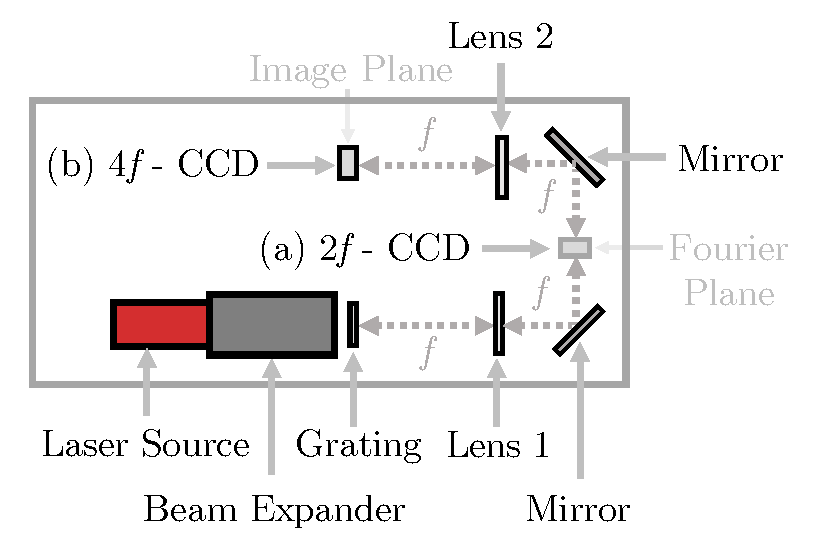
\includegraphics[width=6.5cm]{method/fig1-1}
\caption[]{A plan view schematic of the experimental set-up used to collect data. (a) Represents the main $2f$ optical system used where the majority of data was collected. (b) Represents the 'standard' $4f$ optical system.}
\label{m-fig1}
\end{center}
\end{figure}

Method

\vspace{-3ex}
\section{Results}
\vspace{-2ex}

Results

\begin{figure}[!h]
\begin{center}
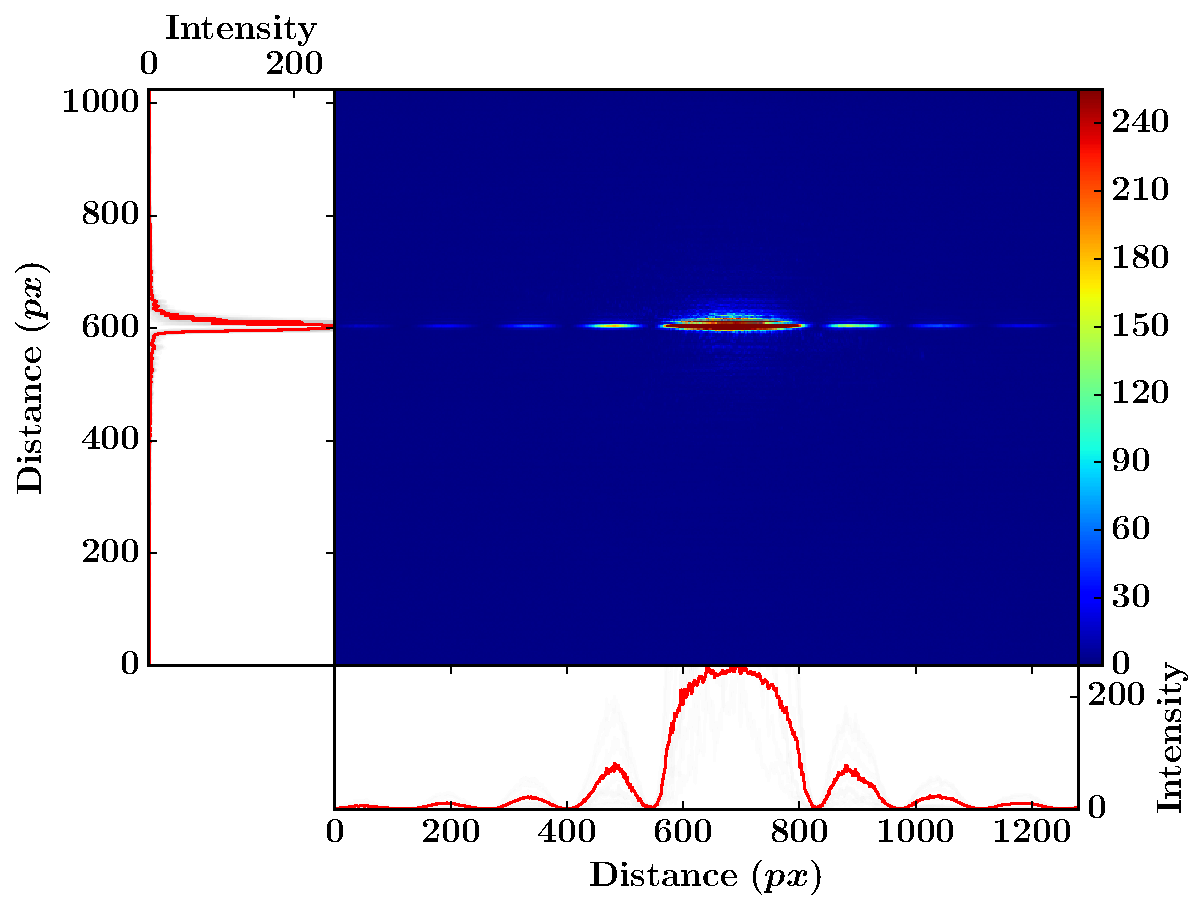
\includegraphics[width=9cm]{results/single_slit}
\caption[]{The intensity profiles in the horizontal and vertical directions for the diffraction pattern of a single slit in the Fourier plane.}
\end{center}
\end{figure}

\begin{table}[h!]
\centering
\begin{tabular}{c@{\hskip 20pt}c@{\hskip 20pt}c@{\hskip 20pt}c} 
 \hline
 \textbf{Grating} & \textbf{Real Space [m]} & \textbf{Fourier Space [m]} \\ [0.5ex] 
 $1$ &$0.55\pm0.03$ & $1.0\pm0.2$ \\ 
 $2$ & $0.47\pm0.03$ & $1.1\pm0.3$ \\
 $3$ & $0.46\pm0.03$ & $1.0\pm0.3$ \\
 \hline
\end{tabular}
\caption{For each coarse diffraction grating, the diffraction grating slit width is shown as measured in real space, and as calculated in Fourier space.}
\end{table}

\vspace{-3ex}
\section{Discussion}
\vspace{-2ex}

Discussion

\vspace{-5ex}
\section{Conclusions}
\vspace{-2ex}

Conclusion

\begin{thebibliography}{5}
\bibitem{mathmethods}
	K. F. Riley, M. P. Hobson, and S. J. Bence.
	\textit{Mathematical Methods for Physics and Engineering}.
	Cambridge University Press, Cambridge, UK, 2010.
	
\bibitem{of2f}
	C. S. Adams and I. G. Hughes.
	\textit{Optics f2f, from Fourier to Fresnel}.
	Clarendon Press, Oxford, UK, 2017.

\bibitem{elecdiffraction}
	K. W. Andrews, D. J. Dyson, and S. R. Keown.
	\textit{Interpretation of Electron Diffraction Patterns}.
	Hilger \& Watts Ltd, London, UK, 1967.
	
\bibitem{xraypharma}
	J. P. Smit, R. B. McClurg.	
	\textit{X-ray Powder Diffraction Pattern Indexing for Pharmaceutical Applications}.
	Pharmaceutical Technology, January 2013, Vol. 37, No. 1.
	
\bibitem{singleslit}
	A. R. Lang, et al.
	\textit{Single-slit diffraction patterns of sub-nanometre-wavelength synchrotron radiation}.
	Journal of Physics D: Applied Physics, 1987, Vol. 20, No. 4, pp. 541-544.
	
\bibitem{xrayphase}
	S. C. Mayo, et al.
	\textit{X-ray phase-contrast microscopy and microtomography}.
	Optical Express, 2003, Vol. 11, No. 19, pp. 2289-2302.

\bibitem{youngandfreedman} 
	Hugh D. Young and Roger A. Freedman.
	\textit{University Physics with Modern Physics, 13th Edition}. 
	Pearson Education Limited, Essex, UK, 2015.
	
	
\bibitem{hughesandhayes} 
	I. G. Hughes and T. P. A. Hase.
	\textit{Measurements and their Uncertainties}. 
	Oxford University Press, Oxford, UK, 2010.
	
\end{thebibliography}
\clearpage

\vfill
\twocolumngrid
\vspace{-3ex}
\section*{Appendix}
\vspace{-2ex}

Appendix


\clearpage
\end{document}